%% ====================================================================
%%  ACT IV: VALIDATION AND PRACTICE (~5pp)
%% ====================================================================
\section{Validation and Practice}
\label{sec:validation}

This section moves from theory to evidence.
We report the decomposition's efficiency advantage over benchmark racing, pair the over-piloting finding with the Bernstein resolution, demonstrate the routing-triviality condition on a worked example, and state when the framework should \emph{not} be used.

\subsection{Efficiency Advantage over Benchmark Racing}
\label{sec:efficiency}

% SOURCE: EXP5
The decomposition-guided procedure selects agent designs at a fraction of the evaluation cost of benchmark racing.
In a synthetic experiment with 5~models, 20~depth levels, and 100~total designs, the decomposition with 100~pilot instances and 50~confirmation instances per mode achieves mean regret~$0.026$---comparable to benchmark racing with 500~evaluations per design (mean regret~$0.029$)---while using $50\times$ fewer total evaluations ($1{,}000$ vs.\ $50{,}000$).

The advantage is measured against benchmark racing at $k = 100$ designs, with break-even at $k \approx 30\text{--}50$.
For small design menus, benchmark racing may be simpler and comparably effective.
For large menus ($k > 50$), the decomposition's cost grows with the number of modes, not the number of designs, making it increasingly advantageous.

\subsection{Over-Piloting and the Bernstein Resolution}
\label{sec:over-piloting}

% SM3: Over-piloting surprise marker
% W7: Over-piloting + Bernstein = single constructive beat
We expected that more pilot data would monotonically improve design selection---at worst, providing diminishing returns.
We were wrong.
The decomposition with 500~pilot instances and 200~confirmations achieves regret~$0.035$, which is \emph{worse} than the configuration with 100~pilots and 50~confirmations (regret~$0.026$).
Beyond a threshold, additional pilot samples refine an already-accurate estimate while consuming budget that is better spent on direct evaluation.

The Bernstein corollary (Corollary~\ref{cor:bernstein}) provides the resolution: it tells practitioners when their estimate is precise enough to stop.
A conservative heuristic: allocate 20--30\% of total evaluation budget to pilot estimation, and use the Bernstein bound to validate this allocation post hoc.
If the Bernstein-required sample size at the observed $\pmin$ is below the actual pilot size, stop piloting.

\subsection{Proxy Validity}
\label{sec:proxy-validity}

% SOURCE_CLAIM: C58
% W2: C58 in Act IV, not Act III
The four-term decomposition operates on expected log certified time, which equals $-\log P_D$ (the negative log success probability) up to a Jensen gap.
A practitioner may worry that this proxy objective selects the wrong design.

\begin{theorem}[Proxy validity]
\label{thm:proxy-validity}
\begin{enumerate}[label=(\alph*)]
  \item For fixed depth~$D$, the proxy $-\log P_D$ and the true objective $\E[\log T]$ rank models identically: $\argmin_M (-\log P_D(M)) = \argmin_M \E[\log T(M)]$.
  \item For fixed model, the cost-adjusted proxy and true objectives have optimizers satisfying $\Dstar_{\mathrm{true}} \le \Dstar_{\mathrm{proxy}}$, with the difference exponentially small in~$\Dstar$.
\end{enumerate}
\end{theorem}

% SM1: Proxy validity surprise marker
We found this genuinely reassuring: the proxy selects the same design.
The 16--28\% absolute gap observed in experiments is a cosmetic Jensen artifact of the form $(1-P_D)/2$, which does not affect which design is selected.
The gap shrinks exponentially with depth and is irrelevant for design ranking.
Full proof in \appref{app:proxy}.

\subsection{Routing Triviality and Ricardian Comparative Advantage}
\label{sec:routing-triviality}

% SOURCE_CLAIM: C60
Before investing in routing infrastructure, a builder should check whether routing adds value at all.

\begin{proposition}[Routing-triviality condition]
\label{prop:routing-triviality}
\begin{enumerate}[label=(\alph*)]
  \item \textbf{Sufficient condition for trivial routing.}
  If for all modes~$s$ and all model pairs $M, M'$:
  $|\log p(s, M) - \log p(s, M')| < |\log \kappa(M) - \log \kappa(M')|$,
  then routing is trivial: the cheapest model wins on every mode.
  \item \textbf{Necessary condition for non-trivial routing.}
  Routing is non-trivial if and only if there exist modes $s_1, s_2$ and models $M_1, M_2$ such that $M_1$ is cost-adjusted-better on $s_1$ but $M_2$ is cost-adjusted-better on $s_2$: different models have different comparative advantages across modes.
\end{enumerate}
\end{proposition}

\begin{remark}[Intermediate regime]
\label{rem:intermediate-routing}
Parts~(a) and~(b) of Proposition~\ref{prop:routing-triviality} precisely delimit when routing matters.
In the intermediate regime where the sufficient condition narrowly fails, we observe numerically that a tighter heuristic bound characterizes routing value; a formal proof remains open.
\end{remark}

The necessary condition is an economic insight: non-trivial routing requires \emph{Ricardian comparative advantage}---different models must be \emph{relatively} better at different task types, not merely absolutely better.
When one model dominates across all modes (the common case with large cost differentials), routing is provably worthless.

\paragraph{Practical pre-check.}
Compute $\Delta_{\mathrm{cost}} = \log(\kappa_{\max}/\kappa_{\min})$ and $\Delta_{\mathrm{comp}} = \max_{s,M,M'} |\log p(s,M) - \log p(s,M')|$.
If $\Delta_{\mathrm{comp}} < \Delta_{\mathrm{cost}}$: routing is trivial, use the cheapest model.
If $\Delta_{\mathrm{comp}} \ge \Delta_{\mathrm{cost}}$: routing may be non-trivial, proceed with full decomposition.
This is a five-minute calculation that can save weeks of engineering.

\textbf{Caveat:} The sufficient condition (part~a) has 62\% accuracy near the boundary where $\Delta_{\mathrm{comp}} \approx \Delta_{\mathrm{cost}}$.
When the competence and cost spreads are within a factor of~2, we recommend the full mode-level check: compute $\rho(s,M) = -\log p(s,M) + \log\kappa(M)$ for all modes and verify whether a single model dominates everywhere.

% W6: EXP8 for main-text four-term bar chart
\paragraph{Worked example (from EXP8).}
In the non-trivial routing scenario with 5~modes, the small model is cost-adjusted-best on modes~1--3 while the large model is cost-adjusted-best on modes~4--5.
The competence spread $\Delta_{\mathrm{comp}} = 3.0$ exceeds the cost spread $\Delta_{\mathrm{cost}} = 1.1$, correctly predicting non-trivial routing.
The information gain under the small model is $G = 0.50$~nats---substantial, because the routing policy can exploit the fact that different models have comparative advantage on different modes.

\begin{figure}[t]
  \centering
  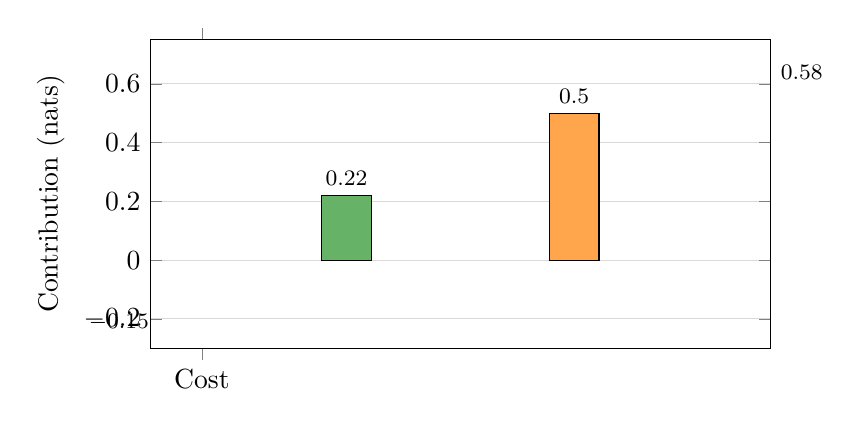
\begin{tikzpicture}
    \begin{axis}[
      ybar,
      bar width=18pt,
      width=0.78\textwidth,
      height=5.5cm,
      ylabel={Contribution (nats)},
      symbolic x coords={Cost,Competence,Info Gain,Mismatch},
      xtick=data,
      ymin=-0.3,
      ymax=0.75,
      ytick={-0.2,0,0.2,0.4,0.6},
      nodes near coords,
      every node near coord/.append style={font=\footnotesize},
      ymajorgrids=true,
      grid style={gray!30},
    ]
    \addplot[fill=blue!40] coordinates {(Cost,-0.15)};
    \addplot[fill=green!50!black!60] coordinates {(Competence,0.22)};
    \addplot[fill=orange!70] coordinates {(Info Gain,0.50)};
    \addplot[fill=red!55] coordinates {(Mismatch,0.58)};
    \legend{}
    \end{axis}
  \end{tikzpicture}
  \caption{Four-term decomposition for the Ricardian scenario (EXP8 data).
  The dominant term is routing mismatch, not competence---indicating that the choice of routing policy matters more than the choice of model in this scenario.
  This is the regime where the full decomposition provides diagnostic value beyond a simple cost comparison.}
  \label{fig:four-term-bar}
\end{figure}

\subsection{Honest Scoping: When NOT to Use This Framework}
\label{sec:scoping}

A framework that does not say when it should not be used is not trustworthy.
The four-term decomposition should not be used when:

\begin{enumerate}
  \item \textbf{Single-mode tasks} ($\Meff \approx 1$): the decomposition reduces trivially to a cost-competence comparison, and a simple A/B test suffices.
  \item \textbf{No pilot data available}: mode discovery is impossible, and the framework is inapplicable.
  \item \textbf{Rapidly shifting task distributions}: the static decomposition becomes stale before it can be exploited.
  \item \textbf{Very small design menus} ($k \le 2$, no depth variation): the framework's overhead exceeds the benefit of a simple comparison.
  \item \textbf{Cost-adjusted homogeneity} (Proposition~\ref{prop:routing-triviality}): when one model cost-dominates on all modes, the routing terms vanish and a cost comparison suffices.
  This condition is formally proved and is checkable from pilot data.
  \item \textbf{Very small $k$} ($k < 30$): the decomposition's efficiency advantage over benchmark racing has not yet materialized.
\end{enumerate}

The cost of running the full framework---approximately \$800 and 4~hours for a 5-model, 8-mode scenario---is justified only when the design menu is large enough ($k > 30\text{--}50$) that benchmark racing becomes prohibitively expensive.

\subsection{Placeholder: Real-Benchmark Validation}
\label{sec:real-benchmarks}

% W9: MI1/MI2 placeholders
To validate generalization beyond synthetic distributions, a natural next step is to apply the framework to established benchmarks.

\paragraph{Formal verification (MI1).}
We plan to instantiate the full pipeline on Lean/Mathlib theorem-proving tasks: define the task distribution, run a pilot study with two models, discover modes via trajectory clustering, estimate the four terms, compute the crossover, and validate the recommendation against a held-out test set.
If the decomposition identifies the same dominant term as in the synthetic setting, this confirms that the geometric-trials assumption and packed-family structure hold on real tasks.

\paragraph{Bayesian optimization baseline (MI2).}
The 50$\times$ advantage is measured against benchmark racing.
The comparison against Bayesian optimization, which can also exploit structure in the design space, is future work.
A GP surrogate with Expected Improvement acquisition, categorical kernel for discrete model choice, and 50-evaluation budget would provide a meaningful baseline.

\subsection{Scaling Advantage}
\label{sec:scaling}

% SOURCE: EXP9
How does the decomposition's advantage grow with the design-menu size?
Analytical predictions suggest the efficiency ratio scales as $k^{0.7\text{--}1.0}$, with break-even at $k \approx 30\text{--}50$.
At $k = 10$, racing uses fewer evaluations ($500$ vs.\ $1{,}400$) and achieves comparable regret.
At $k = 100$, the decomposition uses $2{,}000$ evaluations vs.\ racing's $5{,}000$, with the gap widening as $k$ grows.

We conjecture that the efficiency advantage grows at least as $k^{0.7}$ in the design-menu size, based on analytical predictions that await Monte Carlo confirmation.
If confirmed, this implies that the framework's value increases precisely in the regime where practitioners need it most: large design spaces with many model-routing combinations.
